\documentclass[13pt,a4paper]{article}
\usepackage[spanish,es-nodecimaldot]{babel}	% Utilizar español
\usepackage[utf8]{inputenc}					% Caracteres UTF-8
\usepackage{graphicx}						% Imagenes
\usepackage[hidelinks]{hyperref}			% Poner enlaces sin marcarlos en rojo
\usepackage{fancyhdr}						% Modificar encabezados y pies de pagina
\usepackage{float}							% Insertar figuras
\usepackage[textwidth=390pt]{geometry}		% Anchura de la pagina
\usepackage[nottoc]{tocbibind}				% Referencias (no incluir num pagina indice en Indice)
\usepackage{enumitem}						% Permitir enumerate con distintos simbolos
% \usepackage[T1]{fontenc}					% Usar textsc en sections
\usepackage{amsmath}						% Símbolos matemáticos
\usepackage[ruled,vlined]{algorithm2e}      % Pseudocódigo
\usepackage{xcolor}
\usepackage{listings}
% Para que acepten tíldes los listing
\lstset{     
     literate=%
         {á}{{\'a}}1
         {é}{{\'e}}1
         {í}{{\'i}}1
         {ó}{{\'o}}1
         {ú}{{\'u}}1
         {Á}{{\'A}}1
         {É}{{\'E}}1
         {Í}{{\'I}}1
         {Ó}{{\'O}}1 
         {Ú}{{\'U}}1
         {ñ}{{\~n}}1 
         {Ñ}{{\~N}}1 
         {¿}{{?``}}1 
         {¡}{{!``}}1
}
\usepackage{dsfont}
\usepackage{subfigure}

% ==============================================================================

\usepackage{caption}
\usepackage[section]{placeins}
\makeatletter
\def\fps@figure{H}
\makeatother

\usepackage{booktabs}
\usepackage{longtable}
\usepackage{array}
\usepackage{multirow}
\usepackage{wrapfig}
\usepackage{colortbl}
\usepackage{pdflscape}
\usepackage{tabu}
\usepackage{threeparttable}
\usepackage{threeparttablex}
\usepackage[normalem]{ulem}
\usepackage{makecell}
\usepackage[bottom]{footmisc}

% ==============================================================================
% ==============================================================================

% Comando para poner el nombre de la asignatura
\newcommand{\asignatura}{Big Data II}
\newcommand{\autor}{Ignacio Vellido Expósito}
\newcommand{\email}{ignaciove@correo.ugr.es}
\newcommand{\titulo}{Ejecución paralela en Pig}
\newcommand{\subtitulo}{Práctica sobre ETL}

% Configuracion de encabezados y pies de pagina
\pagestyle{fancy}
\lhead{\autor{}}
\rhead{\asignatura{}}
\lfoot{Máster Ciencia de Datos e Ingeniería de Computadores}
\cfoot{}
\rfoot{\thepage}
\renewcommand{\headrulewidth}{0.4pt}		% Linea cabeza de pagina
\renewcommand{\footrulewidth}{0.4pt}		% Linea pie de pagina

% ==============================================================================
% ==============================================================================

\begin{document}
    \pagenumbering{gobble}
    % ==============================================================================
% Pagina de titulo
\begin{titlepage}
    \begin{minipage}{\textwidth}
        \centering

        
\includegraphics[scale=0.5]{img/ugr.png}\\

        \textsc{\Large \asignatura{}\\[0.2cm]}
        \textsc{MÁSTER CIENCIA DE DATOS E INGENIERÍA DE COMPUTADORES}\\[1cm]

        \noindent\rule[-1ex]{\textwidth}{1pt}\\[1.5ex]
        \textsc{{\Huge \titulo\\[0.5ex]}}
        \textsc{{\Large \subtitulo\\}}
        \noindent\rule[-1ex]{\textwidth}{2pt}\\[2.5ex]

        \end{minipage}

        \vspace{0.3cm}

        \begin{minipage}{\textwidth}

        \centering

        \textbf{Autor}\\ {\autor{} \\ ignaciove@correo.ugr.es}\\[1.5ex]
        \vspace{0.4cm}

        
\includegraphics[scale=0.3]{img/etsiit.jpeg}
        
\includegraphics[scale=0.6]{img/master.png}

        \vspace{0.7cm}
        \textsc{Escuela Técnica Superior de Ingenierías Informática y de Telecomunicación}\\
        \vspace{1cm}
        \textsc{Curso 2020-2021}
    \end{minipage}
\end{titlepage}
% ==============================================================================
    
    \pagenumbering{arabic}    
    \newpage

    % ==============================================================================

\section{Experimento}

Dataset con medidas de peticiones en la red de una universidad, publicado en la página de la UCI (\url{https://archive.ics.uci.edu/ml/datasets/Internet+Firewall+Data}). Cuenta con 65.532 instancias y los siguientes 12 atributos:
\begin{itemize}
    \item Source Port
    \item Destination Port
    \item NAT Source Port
    \item NAT Destination Port
    \item Action (cuatro tipos: allow, action, drop y reset-both)
    \item Bytes
    \item Bytes Sent
    \item Bytes Received
    \item Packets
    \item Elapsed Time (sec)
    \item pkts\_sent
    \item pkts\_received
\end{itemize}

\subsection{Pasos para el desarrollo del experimento}

Tras descargar el .csv, debemos cargarlo en HDFS.
\begin{lstlisting}    
    $ mv Downloads/log2.csv /var/tmp/materialPig/log2.csv
\end{lstlisting}

\vspace{\baselineskip}

Creamos el directorio en HDFS:
\begin{lstlisting}
    $ hdfs dfs -mkdir input
\end{lstlisting}

\vspace{\baselineskip}

Cargamos los datos en el directorio:
\begin{lstlisting}
    $ hdfs dfs -put /var/tmp/materialPig/log2.csv input
\end{lstlisting}

\vspace{\baselineskip}

Entramos en Pig:
\begin{lstlisting}
    $ pig
\end{lstlisting}

\newpage

Creamos esquema del flujo del que leer los datos:
\begin{lstlisting}
    > measure = load 'input/log2.csv' 
                using PigStorage(',') 
                as (
                    SourcePort:int ,
                    DestinationPort:int ,
                    NATSourcePort:int ,
                    NATDestinationPort:int ,
                    Action:chararray,
                    Bytes:int ,
                    BytesSent:int ,
                    BytesReceived:int ,
                    Packets:int ,
                    ElapsedTime:int ,
                    pktsSent:int ,
                    pktsReceived:int
                );
\end{lstlisting}

\vspace{\baselineskip}

Aplicamos la consulta: \textbf{Calcular la cantidad máxima de bytes enviados y la carga media por paquete 
(en cualquier puerto de destino) para aquel puerto con más solicitudes al 
puerto HTTPS (443)}

\vspace{\baselineskip}

1. Seleccionamos las peticiones a HTTPS:
\begin{lstlisting}
    > all_ports = foreach measure generate DestinationPort, SourcePort;
    > https_ports = filter all_ports by DestinationPort==443;
\end{lstlisting}

\vspace{\baselineskip}

2. Agrupamos por puerto de origen y calculamos el que ha realizado más peticiones:
\begin{lstlisting}
    > ports = group https_ports by SourcePort ;
    > groups = foreach ports generate group, COUNT(https_ports) as count;
    > max_port = limit (order groups by count desc) 1;
\end{lstlisting}

\vspace{\baselineskip}

\begin{figure}[H]\center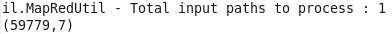
\includegraphics[width=.65\linewidth]{img/1.png}\end{figure}

(Hace falta renombrar COUNT para hacerle referencia en la expresión siguiente)

\newpage

3. Filtramos peticiones por puerto de origen y calculamos la información solicitada
\begin{lstlisting}
    > petitions = filter measure by SourcePort==max_port.group;
    > out = foreach (group petitions by SourcePort) 
            generate group, 
                      MAX(petitions.BytesSent), 
                      (float)(SUM(petitions.BytesSent)/SUM(petitions.Packets));
\end{lstlisting}

\vspace{\baselineskip}

(Aunque todas las peticiones sean del mismo puerto, agrupamos para poder mostrarlo con facilidad)

\vspace{\baselineskip}

4-1. Podemos mostrar el resultado con:
\begin{lstlisting}
    > dump out;
\end{lstlisting}

\vspace{\baselineskip}

4-2. O guardarlo con:
\begin{lstlisting}
    > store out into 'pigResults/firewall' using PigStorage(',');;
\end{lstlisting}

\begin{figure}[H]\center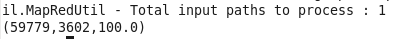
\includegraphics[width=.95\linewidth]{img/2.png}\end{figure}

    \setlength{\parskip}{1em}
    
    % ==============================================================================
    
    \newpage
\end{document}

% ==============================================================================
% ==============================================================================